\documentclass[12pt,twoside]{report}
% Die Option a4paper kann nötig sein, um das PDF nachher beim Copyshop drucken zu können.
%\documentclass[12pt,twoside,a4paper]{report}


\makeindex
\usepackage{german,a4}
\usepackage{color}
%\usepackage[dvips]{graphicx}
\usepackage{psfrag}
\usepackage{epsfig}
\usepackage[utf8]{inputenc}
\usepackage{fancyhdr}
\usepackage{caption}
\usepackage{cite}
\usepackage{graphicx}
% setzt den pfad zum suchen der bilder
\graphicspath{{figures/}}
\usepackage{subcaption}
%\usepackage{subfig}
\usepackage{float}
\usepackage{pgfplots}
\pgfplotsset{compat=newest}
%% the following commands are needed for some matlab2tikz features
\usetikzlibrary{plotmarks}
\usetikzlibrary{arrows.meta}
\usepgfplotslibrary{patchplots}
\usepackage{amsmath}
\usepackage{textcomp}

\usepackage[svgnames,pdf]{pstricks}
\usepackage{pst-grad} % For gradients 
\usepackage{pst-plot} % For axes 
\usepackage[space]{grffile} % For spaces in paths 
\usepackage{etoolbox} % For spaces in paths
\usepackage{pgf,tikz}
\usetikzlibrary{arrows}
\usepackage{tabularx}

\usepackage{url}
\usepackage{listings}
\usepackage{pdfpages}
\usepackage{subcaption}
\makeatletter % For spaces in paths 
 \patchcmd\Gread@eps{\@inputcheck#1 }{\@inputcheck"#1"\relax}{}{} 
 \makeatother


\usepackage{listings}
\usepackage{color}
\definecolor{lightgray}{gray}{0.9}

\lstset{
    showstringspaces=false,
    basicstyle=\ttfamily,
    keywordstyle=\color{blue},
    commentstyle=\color[grey]{0.6},
    stringstyle=\color[RGB]{255,150,75}
}

\newcommand{\inlinecode}[2]{\colorbox{lightgray}{\lstinline[language=#1]$#2$}}

\include{makros}



%Definition der Seitengr"osse
\setlength{\textwidth}{15.5 true cm}
\setlength{\textheight}{22 true cm}

\oddsidemargin  0.5 cm
\evensidemargin 0.5 cm
\topmargin      0 cm
\parindent 			0 cm

\selectlanguage{german}



\renewcommand{\baselinestretch}{1.5}
 \renewcommand{\captionfont}{\linespread{1}\normalsize} 
 \renewcommand{\textfraction}{0}

% Fancyhdr
\setlength{\headheight}{0.75cm}
\fancypagestyle{plain}{
	\fancyhf{}
	\fancyhead[EL,OR]{\thepage}
	\fancyhead[ER]{\leftmark}
	\fancyhead[OL]{\leftmark}
	}

\fancypagestyle{newfancy}{
	\fancyhf{}
	\fancyhead[EL,OR]{\thepage}
%	\fancyhead[ER]{\rightmark}
	\fancyhead[OL]{\rightmark}
	}
\pagestyle{newfancy}


\renewcommand{\chaptermark}[1]{\markboth{\uppercase{\chaptername \ \thechapter.\ #1}}{}} 
\renewcommand{\sectionmark}[1]{ \markright{ \uppercase{\thesection.\ #1}}{}} 




\begin{document}


%%%%%%%%%%%
%  Titel  %
%%%%%%%%%%%

\begin{titlepage}
\begin{center}
\vspace*{-1cm}
 {\LARGE Friedrich-Alexander-Universität Erlangen-Nürnberg}\\
\vspace{1cm}  
 {\Large \textbf{Lehrstuhl für Rechnerarchitektur}}\\
\vspace{1cm}  
 {\Large Prof. Dr. Dietmar Fey}\\
\vspace{3cm}  
 {\LARGE Masterprojekt}\\
\vspace{2cm}  
 {\LARGE \textbf{Smartcameras\\ Detektion von Straßenschildern und Pylonen mittels Viola-Jones Algorithmus}}\\
\vspace{2cm} 
{\LARGE von Christoper Werner\\und \\ Maximilian Langohr}\\
\vspace{3cm} 
{\Large März 2018}\\
\vspace{1cm} 
{\Large }

\end{center}
\end{titlepage}


%\addtocounter{page}{-1} 





%%%%%%%%%%%%%%%%%%%%%%%%
%  Inhaltsverzeichnis  %
%%%%%%%%%%%%%%%%%%%%%%%%
\addtocounter{page}{-2}
\tableofcontents   
\clearpage

%%%%%%%%%%%%%%%%%
%  Kurzfassung  %
%%%%%%%%%%%%%%%%%

%\renewcommand{\chaptermark}[1]{ \markboth{ \uppercase{#1}}{}} 
%\input{emptypage}
%\chaptermark{Kurzfassung}
%\renewcommand{\chaptermark}[1]{\markboth{\uppercase{\chaptername \ \thechapter.\ #1}}{}} 

%\chapter*{Kurzfassung}
%\addcontentsline{toc}{chapter}{Kurzfassung}
%Kurzfassung
%\clearpage

%%%%%%%%%%%%%%%%
% Ausarbeitung %
%%%%%%%%%%%%%%%%

% Abstände vor und nach Formeln
\setlength{\belowdisplayskip}{0.5cm}
\setlength{\belowdisplayshortskip}{0.5cm}
%\setlength{\abovedisplayskip}{-0.05cm}
%\setlength{\abovedisplayshortskip}{-0.05cm}

\renewcommand{\sectionmark}[1]{ \markright{ \uppercase{\chaptername \ \thechapter.\ #1}}{}} 
\chapter{Motivation}
\sectionmark{Danksagung}
\chaptermark{Motivation}
\sectionmark{Motivation}
\label{chap:Motivation} 
\pagenumbering{arabic}
Autonomes Fahren ist eines der großen Themen der Automobilindustrie der letzten Jahre. Der Traum vom eigenständig fahrenden Auto besteht schon länger, jedoch gestaltet sich die komplett selbstverwaltende Fahrzeugsteuerung als schwierig, da unheimlich viele Faktoren miteinbezogen sowie analysiert werden müssen.\\
Einer dieser Faktoren ist die erfolgreiche und korrekte Erkennung von Straßenschildern sowie wegweisenden Objekten, in diesem Fall Verkehrshütchen. Ansätze hierzu gibt es viele, jedoch ist die Forschung der Automobilindustrie meist geheim, weshalb eigene Ansätze kreiert werden müssen.\\
Dieses Projekt stellt den Versuch da, sich diesem Thema mit einer Methode zu nähern. Das Projekt verfolgte die Verwirklichung von Zwei Anforderungen:
\begin{enumerate}
\item Es sollen zwei nebeneinanderstehende Verkehrshütchen, auch Pylonen genannt, korrekt erkannt werden und die Position der erkannten Objekte im Bild zurückgegeben werden.
\item 3 Arten von Verkehrszeichen, das Stopschild, Vorfahrt gewähren sowie das Vorfahrtszeichen sollen erkannt werden.
\end{enumerate}
Das Ziel, was hierbei verfolgt wird ist, dass einerseits die Erkennung von Pylonen dazu genutzt werden kann einen Parcours aufzustellen, durch den das Auto eigenständig navigiert, sowie die Erkennung von Verkehrszeichen auf einer Teststrecke für korrektes Fahrverhalten genutzt werden kann. Die Voraussetzung ist, dass dazu der Algorithmus von Viola und Jones , welcher in einem Paper im Jahr 2001 vorgestellt wurde, für diesen Anweundgsfall adaptiert und genutzt wird.
\renewcommand{\sectionmark}[1]{ \markright{ \uppercase{\thesection.\ #1}}{}} 

%%%%%%%%%%%%%%%%
% Viola-Jones  %
%%%%%%%%%%%%%%%%

\chapter{Der Viola und Jones Algorithmus}
\chaptermark{Viola-Jones}
\label{chap:viola-jones}
In diesem Kapitel gilt es die Rahmenbedingungen für das erfolgreiche Nutzen des Viola-Jones Algrithmus abzustecken. Hierbei werden die Schritte für die Vorbereitungen erklärt und ein grober Überblick über den Ablauf mit detailreicheren Erklärungen für die interessanten Teilgebiete gegeben. Abschließend wird auf die Probleme, die bei dem Ablauf des Algorithmus entstehen können, eingegangen.

\section{Vorbereitungen und grundlegender Ablauf}
Die Liste an Vorbereitungen gliedert sich wie folgt:
\begin{itemize}
\item[] \textbf{Zu erkennendes Objekt}\\ Es ist eine klare Vorstellung vom Objekt notwendig, wie dieses auszusehen hat und in welchen Situationen, also beispielswiese verschiedenen Winkeln und Lichtverhältnissen, dieses vorkommen kann.
\item[] \textbf{Bilddatenbanken}\\ Eine Datenbank an Negativbildern ist für den Algorithmus unabdingbar. Je größer die Datenbank ist, desto besser. Jedoch ist ein Limit von 10,000 bildern empfehlenswert, da der Trainingsprozess ansonsten zu lange dauert. Eine Datenbank an Positivbildern ist nicht zwingend erforderlich und hängt von der Art des zu erkennenden Objekts ab. Ist das Objekt ein rigides Objekt reichen wenige Positivbilder, um das Training erfolgreich durchführen zu können. Im Falle eines nicht-rigiden Objekts, beispielsweise eines Gesichtes, ist es wichtig möglichst viele Formen und Farben zu haben, weshalb eine Datenbank an positiven Bildern notwendig ist.
\item[] \textbf{Geeignete Datei- und Ordnerstruktur}\\ Die Ordnerstruktur, in der die Bilder und Ergebnisse des Trainings abgelegt werden, sollte von vornherein durchdacht sein. In der Ordnerstruktur sollten sich jeweils ein Ordner für die positiven Bilder, einer für die negativen Bilder sowie ein Ordner für die zu speichernden Ergebnisse befinden. Auf der gleichen Ebene, auf der sich diese Ordner befinden sollten die Textdateien für die Pfade zu den Hintergrundbildern, Pfade zu den positiven Bilder, das Vectorfile mit Informationen über alle positiven samples in den positiven Bildern und das info File mit Informationen über das Vorkommen des Objekts in den positiven Bildern befinden.
\item[] \textbf{Programm zum Antrainieren}\\ Das in diesem Projekt verwendete Programm ist eine OpenCV-implementierung, die auf dem Raspberry PI kompiliert wurde. OpenCV liefert 3 weitere Tools, die zum Antrainieren der Klassifizierer verwendet wurden. Genaueres hierzu ist im Abschnitt \ref{sec:Antrainieren} zu finden.
\item[] \textbf{Rapsberry PI mit ROS}\\ Für dieses Projekt wurde ein Raspberry PI 3 Modell B 1.2 verwendet. Das Betriebssystem ROS wurde auf eine Micro-SD Karte gespielt und lief standardmäßig auf dem Raspberry PI.
\item[] \textbf{Optional: Kamera und Bildbearbeitungstool}\\ In unserem Fall wurden alle positiven Samples mit einer Canon EOS 600D aufgenommen. Die anschließende Bearbeitung der Bilder erfolgte mit Photoshop CC. Hierbei wurden die Bilder zurechtgeschnitten, Hintergründe geglättet und Unreinheiten im Bild beseitigt.
\end{itemize}
Der allgemeine Ablauf besteht aus der Vorbereitung der Trainingsdaten und Kaskadentraining. Diese beiden Hauptthemen können jedoch noch feiner untergliedert werden. Die Untergliederung für die Vorbereitung der Trainingsdaten sieht wie folgt aus:
\begin{enumerate}
\item \textbf{Erstellen der Liste der Negativbilder}\\ Die Liste negativer Bilder wird über den Befehl
\begin{lstlisting}
find negative/ -iname "*.jpg" > bg.txt
\end{lstlisting}
von uns erstellt. Dieser Befehl extrahiert sämtliche jpg-Dateinamen aus dem Verzeichnis '/negative' und schreibt diese in das Textfile 'bg.txt'
\item \textbf{Erstellen der Liste der Positivbilder}\\ Die Liste der Positivbilder wird in der Regel per Tool erstellt, da diese ebenfalls die Objektvorkommnisse im Bild enthalten muss.
\end{enumerate}
Anschließend gilt es die erstellten Trainingsdaten zu verwerten:
\begin{enumerate}
\item \textbf{Erstellen von positiven Samples}\\ Positive Samples werden erstellt, indem das Tool Opencv\_createsamples mit den entsprechenden Kommandoparametern gestartet wird. Hierbei wird die Datenbank an positiven Bildern erstellt, aus der anschließend das positive Vectorfile erstellt wird. Die hierbei erstellten Bilder unterscheiden sich von den rein positiven Bildern, da diese Bilder eine Kombination aus rein positiven Bildern und negativen Bildern darstellen und somit eine realere Situation für das Vorkommen eines Objektes im Bild darstellen.
\item \textbf{Erstellen des positiven Vectorfiles}\\ Das positive Vectorfile fasst sämtliche Vorkommnisse von Objekten in den positiven Samples aus vorherigem Schritt in einem File zusammen. Dieses File ist essenziell für den weiteren Trainingsprozess.
\item \textbf{Kaskadentraining}\\ Als letzter Schritt im Ablauf gilt das Antrainieren der Kaskaden. Hierbei wird das positive Vectorfile verwendet um in verschiedenen Stages mit schwachen Klassifizierern, auch weak classifiers, eine Kaskade zu erstellen, die das Objekt möglichst einwandfrei erkennt.
\end{enumerate}
Nach der groben Beschreibung des Prozesses erfolgt nun die Erläuterung der einzelnen und wichtigeren Teilschritte in den folgenden Abschnitten.


\section{Antrainieren der Klassifizierer}
\subsection{Voraussetzungen}
Um einen Klassifizierer für den Viola Jones Algorithmus anlernen zu können, braucht dieser folgende Dinge:
\begin{enumerate}
\item Einen Datensatz an originalen positiven Bildern. Positiv heißt, dass in diesem Bild das zu erkennende Objekt enthalten ist.
\item Optional: Einen Datensatz an künstlichen positiven Bildern. Dieser kann mit entsprechenden Tools aus obigen originalen positiven Bildern und einem Datensatz an Negativbildern erzeugt werden.
\item Zu dem Datensatz mit positiven Bildern muss es eine Liste geben, die alle Vorkomnisse an Objekten in einem positiven Bild enthält. Diese wird meist als 'info.txt' abgespeichert und entspricht der Form \\
\textbf{[Verzeichnis/Bildname] [Anzahl vorkommender Objekte] [X-Position Y-Position Breite Höhe]}. \label{sec:info_txt}\\
Wobei der Ursprung des Koordinatensystem in der linken oberen Ecke ist und das Koordinatensystem sich über die normalerweise negative Y-Achse aufspannt.
\item Ein Datensatz an negativen Bildern. Negativ bedeutet, dass in diesem Bild das zu erkennende Objekt nicht enthalten ist. Es kann also irgendein wahlfreies Bild sein, ohne das Vorkommen des Objekts. Hierzu muss ebenfalls eine Liste erstellt werden, die alle Bilder vereint. Diese Liste wird in der Regel 'bg.txt' genannt. Die Form hierfür ist \\
\textbf{[Verzeichnis/Bildname]}.
\item Ein Programm, mit dem ein Haar-like Klassifizierer angelernt werden kann. Das in dieser Arbeit verwendete Programm ist OpenCV.
\end{enumerate}
Die Anzahl an zu verwendenden Bildern wurde absichtlich weggelassen. Dies liegt daran, dass die Anzahl an benötigten Bildern stark variieren kann und vom Objekt abhängt. Im Beispiel eines rigiden Objekts können gute Ergebnisse mit wenigen Originalbildern erzielt werden, in unserem Fall ein Verkehrspylon. Im Falle eines nicht-rigiden Objekts, beispielsweise einem Gesicht, kann es wesentlich mehr Abweichungen von der Norm geben, weshalb eine wesentlich größere Anzahl an originalen Positivbildern erzeugt werden muss. \\
Hat man obige Kriterien erfüllt, kann mit dem Lernprozess begonnen werden.

\subsection{Antrainieren}
Der Prozess des Antrainierens gestaltete sich zu Anfangs sehr schwierig. Das Problem hierbei war, dass die Dokumentation durch OpenCV an Stellen teils sehr dürftig ist. \\
Die grundlegenden Schritte des Antrainierens eines Klassifizierers werden im Folgenden genau erörtert.
\label{sec:Antrainieren}

\subsubsection{Opencv Annotations}
Der erste Schritt zum Antrainieren qualifizierter Klassifizierer ist eine simple Vorbereitung der zu verwendenden Bilder, bei der es darum geht, die zu erkennenden Objekte in einem Bild zu markieren. Die Verwendung ist wie folgt:
\begin{lstlisting}
opencv_annotations -annotations [info.txt] -images [Bilder]
\end{lstlisting}
Dieses Tool öffnet die in '-images' spezifizierten Bilder. Als Paramter kann hier ein Ordner, aus dem dann alle Bilder sequentiell geöffnet werden, oder eine einzelne Bilddatei angegeben werden. Die Angabe '[info.txt]' ist hierbei die Datei, in der die entsprechenden Angaben niedergeschrieben werden. Das gespeicherte Format wurde bereits im Abschnitt \ref{sec:info_txt} erklärt. \\
Startet man das Programm via Konsole, erscheint ein Fenster in dem das spezifizierte Bild, bzw. das erste Bild im Ordner, angezeigt ist. Mit dem ersten Linksklick wird die Aufnahme der annotation gestartet. Das Bewegen der Maus erzeugt ein rotes Rechteck, dass vom ursprünglichen Mausklickpunkt startet. Ist das Rechteck korrekt gezogen, bestätigt ein zweiter Mausklick das gezogene Rechteck. Die Eingabe wird mit 'c' bestätigt. Werden anschließend weitere Objekte im Bild markiert, wird das vorherige rote Rechteck grün gefärbt. Dies indiziert, dass das Rechteck gespeichert wurde. Die gespeicherte Eingabe kann nicht mehr rückgängig gemacht werden.\\
Bei Eingabe von 'n' wird das nächste Bild im Ordner geladen, falls ein Ordner angegeben wurde, ansonsten wird der Prozess beendet und die Info Datei mit den entsprechenden Paramtern erstellt.

\subsubsection{Opencv Createsamples}
Der zweite Schritt des Antrainierens ist der wichtigste. Hier werden die Samples, mit denen später die Haar-like Features gebildet werden, erstellt. Die Algorithmus ist vielseitig verwendbar, da er verschiedene Kombinationsmöglichkeiten der Paramter betrachtet und anhand derer Samples erstellt.\\
In dieser Arbeit werden nur die Fälle vorgestellt, die zum erstellen der Samples verwendet wurden. Die erste Methode diente zur Erstellung künstlicher Samples.
\begin{lstlisting}
opencv_createsamples -img Vorfahrtsschilder/Vorfahrt2.png
\end{lstlisting}
\begin{lstlisting}
-info info.txt -bg bg.txt -num 1000 -maxidev 40
\end{lstlisting}
\begin{lstlisting}
-maxxangle 0.2 -maxyangle 0.2 -maxzangle 0.2 -w 32 -h 32
\end{lstlisting}
\begin{lstlisting}
-bgcolor 125 -bgthresh 10 -show
\end{lstlisting}
Obiger Befehl ist ein Beispiel, dass in dieser Form zur Erstellung von Samples für das zweite Vorfahrtsschild verwendet wurde. Die einzelnen Komponenten ergeben sich wie folgt:
\begin{table}[H]
\begin{tabularx}{\textwidth}{|c|X|}
\hline
Parameter & Erklärung \\ \hline
img & Beschreibt das Bild, welches für die Erstellung der künstlichen Bilder als Grundlage dient. Dieses Bild muss cropped vorliegen. Der Hintergrund muss eine einheitliche Farbe sein, damit das Bild in die Negativbilder ohne Rand oder ähnliches eingebettet werden kann.\\ \hline
info & Spezifiziert den Speicherort, an den die Informationen für die generierten Bilder geschrieben werden. Die Datei wird, falls vorhanden, überschrieben. Sie enthält anschließend zu jedem generierten Bild die Bounding Box für das Objekt in diesem Bild.\\ \hline
bg & Ist die Datei in der die Auflistung der Negativbilder steht.\\ \hline
num & Gibt die Anzahl an positiven Samples an, die erstellt werden soll.\\ \hline
maxidev & Gibt die maximale Abweichung des Intensitivitätsgrads an.\\ \hline
maxXYZangle & Maximale Drehung in RAD die für das Erstellen der Samples verwendet wird.\\ \hline
w und h & Geben die Breite und Höhe in Pixel an. Diese Werte sollten entsprechend der Form des Objekts gewählt werden. Beispielsweise bei einem Cone wird circa ein Seitenverhältnis von 1:2 vorhanden sein, weshalb die Höhe zweimal so groß wie die Breite sein sollte.\\ \hline
bgcolor & Gibt den Wert für die Hintergrundfarbe an. Am besten ist eine schwarze oder weiße Hintergrundfarbe, da bgcolor dann auf 0 bzw 255 gesetzt werden kann. Bei richtig gesetztem Wert wird der Hintergrund in der Sample Erstellung transparent.\\ \hline
\end{tabularx}
\end{table}

\begin{table}[H]
\begin{tabularx}{\textwidth}{|c|X|}
\hline
bgthresh &  Der Abweichungswert für die bgcolor Erkennung. Dieser Wert sollte möglichst klein (Maximal 10) sein, um nicht andere Bereiche des Objekts versehentlich als transparent darzustellen.\\ \hline
show & Ist dieser Parameter gesetzt werden Bilder, bevor sie erstellt werden, angezeigt. Es kann folglich überprüft werden, ob Werte wie bgcolor oder mögliche Winkel richtig gesetzt sind und somit das Sample korrekt in die Negativbilder eingebettet wird. \\ \hline
\end{tabularx}
\label{tab:createsamples parameters}
\caption{Opencv Createsamples: Parameter und deren Erklärung}
\end{table}
Die obige Anwendung des Programms zeigt, wie künstliche Samples zum anlernen erstellt werden können. Der eigentliche Zweck des Programms ist es jedoch sogenannte Vectorfiles zu erstellen. Diese Vector Files sind für den Lernprozess essenziell, da sie die Vektordaten  darüber enthalten, wo die zu erkennenden Objekte in den positiven Bildern liegen. Diese Datei wird anschließend für das antrainieren der Kaskaden genutzt. Der Befehl zum Erstellen dieser Datei sieht wie folgt aus:
\begin{lstlisting}
opencv_createsamples -info info.txt -bg bg.txt
\end{lstlisting}
\begin{lstlisting}
-num 3000 -vec pos.vec
\end{lstlisting}
\begin{table}[H]
\begin{tabularx}{\textwidth}{|c|X|}
\hline
Parameter & Erklärung \\ \hline
info & Spezifiziert den Speicherort, aus dem die Informationen zu den positiven Bildern geladen werden.\\ \hline
bg & Gibt erneut die Speicherposition der Negativbilder an.\\ \hline
num & Anzahl an positiven Samples, die erstellt wird.\\ \hline
vec & Speicherort, an dem die Ausgabe des Programms in Form eines vector Files stattfindet.\\ \hline
\end{tabularx}
\label{tab:createsamples parameters2}
\caption{Opencv Createsamples: Parameter und deren Erklärung für die 2. Variante}
\end{table}
\label{sec:opencv_createsamples}

\subsubsection{Opencv Traincascade}
Im letzten Schritt zum Antrainieren der Klassifizierer wird das Tool 'opencv traincascade' verwendet. Dieses Programm dient dazu, die in den vorherigen Schritten erstellten Samples zum antrainieren eines Klassifizierers zu verwenden. Eine beispielhafte Verwendung sieht wie folgt aus:
\begin{lstlisting}
opencv_traincascade -data obj-classifier/ -vec pos.vec 
\end{lstlisting}
\begin{lstlisting}
-bg bg.txt -numPos 2800 -numNeg 2800 -minHitRate 0.999 
\end{lstlisting}
\begin{lstlisting}
-maxFalseAlarmRate 0.5 -numStages 14 -numThreads 8 
\end{lstlisting}
\begin{lstlisting}
-featureType HAAR -mode ALL -w 32 -h 32 
\end{lstlisting}
\begin{lstlisting}
-precalcValBufSize 4096 -precalcIdxBufSize 4096 
\end{lstlisting}
\begin{lstlisting}
-nonsym -baseFormatSave
\end{lstlisting}
Es ist offensichtlich, dass dieser Befehl eine Fülle an Optionen zum antrainieren mit sich bringt. Im Folgenden wird nur auf die wichtigsten und elementaren Aspekte dieses Befehls eingegangen.
\begin{table}[H]
\begin{tabularx}{\textwidth}{|c|X|}
\hline
Parameter & Erklärung \\ 
\hline
data & Im '-data' Abschnitt wird der Ordner festgelegt, in welchen die Stages, ein sogenanntes 'params.xml' File und die Kaskade abgelegt werden. Nach jeder Stage im Trainingsprozess wird ein neues File namens 'stageX.xml', wobei 'X' für die entsprechende Stage steht, in dem '-data' Ordner angelegt. Sollte das Training erfolgreich sein, indem der Prozess entweder bis zur in '-numStages' gesetzten Stage gekommen ist oder die entsprechende Erfolgsrate erreicht hat, wird ein File namens 'cascade.xml' erzeugt. Dieses File kann vom Viola-Jones Algorithmus genutzt werden. Das 'params.xml' File ist ein einfaches XML Konstrukt, dass einige Paramater, welche in obiger Codezeile verwendet wurden, speichert, um diese bei einer Fortsetzung des Trainings wiederverwenden zu können. Dies bedeutet natürlich auch, dass sobald der Trainingsprozess mit gesetzten Parametern begonnen wurden, diese nicht mehr geändert werden können. Außnahmen hierzu werden im an diese Tabelle folgenden Abschnitt erklärt. \\ 
\hline
vec & Gibt den Pfad zum pos.vec File, welches im Abschnitt  \ref{sec:opencv_createsamples} bereits erklärt wurde, an.\\ 
\hline
bg & Gibt den Pfad zur bg.txt Datei an.\\ \hline
\end{tabularx}
\end{table}

\begin{table}[H]
\begin{tabularx}{\textwidth}{|c|X|}
\hline
numPos & Legt die Anzahl an positiven Samples fest, die für die Stage 0 verwendet werden. Hierbei ist zu beachten, dass je nach Anzahl an zu trainierende Stages ein Wert unterhalb des Limits an positiven Samples, die in pos.vec im vorherigen Schritt generiert wurden, gewählt werden muss. Dies liegt daran, dass pro Stage zusätzliche positive Samples mit in Betracht gezogen werden. Der Grund hierfür ist, dass das Trainingsergebnis auch mit Samples funktionieren soll, mit denen nicht gelernt wurde, also eine automatische Überprüfung der Zwischenergebnisse. Der Wert für '-numPos' sollte maximal entsprechend der Hitrate gewählt werden. Beispielsweise werden bei einer minHitrate von 0.99 pro Stage circa 1\% positive Samples für den Trainingsprozess hinzugezogen. \\ 
\hline
numNeg & Gibt die Zahl an negativen Bildern an. Die Zahl darf nicht größer als die Anzahl an Bildern in der 'bg.txt' Datei sein. In manchen Fällen ist es ratsam, einen kleineren Wert an Negativbildern zu wählen, in der Regel sollte der Wert jedoch genau der Anzahl an Samples in der 'bg.txt' Datei entsprechen. \\ 
\hline
minHitRate & Setzt die Mindestrate, mit der die positiven Bilder erkannt werden müssen. Bei obigem Beispiel ist die minHitRate auf 0.999 gesetzt, was bedeutet, dass der Trainingsprozess trotzdem erfolgreich ist, wenn 1 aus 1000 Objekten nicht erkannt wurde. Die minHitRate hat direkten, aber nicht proportionalen, Einfluss darauf, wieviele neue positive Samples für die nächste Stage zum trainieren verwendet werden. \\ 
\hline
\end{tabularx}
\end{table}

\begin{table}[H]
\begin{tabularx}{\textwidth}{|c|X|}
\hline
maxFalseAlarmRate & Gibt die Rate an, wieviele Weak Classifier einen sogenannten False Positive, also eine vermeintliche korrekte Erkennung des entsprechenden Bildabschnitts, abgeben dürfen. 0.5 entspricht dem Standardwert. Experimente mit diesem Wert wurden nicht unternommen, da alle Ergebnisse mit diesem Wert erzielt wurden.\\ 
\hline
numStages & Dieser Wert gibt an, bis zu welchem Grad das Training ausgeführt werden soll. Je mehr Stages, desto genauer ist das Ergebnis, also der Klassifizierer. Jedoch kann es passieren, dass im Falle einer zu hoch gewählten Anzahl an Stages das Ergebnis 'Overfitted' ist, also der Klassifizierer nicht mehr allgemein genug ist. Hierbei kann dann das Objekt nur unter ganz bestimmten Bedingungen korrekt erkannt werden. Die AcceptanceRatio ist ein Anhaltungspunkt anhand derer eine passende Anzahl an maximale Anzahl an Stages gewählt werden kann. Die AcceptanceRatio wird nach der Befehlserklärung erklärt.\\ 
\hline
numThreads & Für den Falle, dass Multithreading auf der Maschine zur Verfügung steht, kann dieser Parameter gesetzt werden. Multithreading führt zu einer deutlichen Zeitersparnis beim Antrainieren des Klassifizierers.\\ 
\hline
featureType & Für unser Training wurden Haar-like Features verlangt, weshalb dieser Parameter auf 'HAAR' gesetzt wurde. Andere Featuretypen wie beispielsweise LDBP wären ebenfalls möglich, waren jedoch nicht Gegenstand dieses Projekts.\\ 
\hline
mode & Dieser Parameter gibt die zulässigen Weak Classifier an. Es stehen die Modi 'BASIC', 'CORE' und 'ALL' zur Verfügung. Der Modus 'ALL' war bei uns eine zwingende Wahl, da unsere Objekte schräge Kanten enthalten und nur dieser Modus die entsprechenden Weak Classifier hierzu anwendet.\\ 
\hline
\end{tabularx}
\end{table}

\begin{table}[H]
\begin{tabularx}{\textwidth}{|c|X|}
\hline
w und h & Geben die Größe, in Form von Breite und Höhe, der in pos.vec spezifizierten Samples an. Die Werte müssen zwingend den Werten der genutzten Samples entsprechend, da das Programm sonst den Trainingsprozess nicht durchführen kann.\\ 
\hline
precalcValBufSize & Genutzer Buffer im Hauptspeicher um Vorberechnungen auszulagern und den Trainingsprozess zu beschleunigen. Ein Wert von mindestens '1024' sollte hier gewählt werden, um eine Beschleunigung zu erreichen.\\ 
\hline
precalcIdxBufSize & Entsprechend dem Vorgänger sollte dieser Parameter den gleichen Wert erhalten, um eine Beschleunigung zu erzielen. Dieser Parameter muss implizit genutzt werden, sollte '-precalcValBufSize' genutzt werden.\\  \hline
nonsym & Lässt man diesen Parameter weg, wird die params.xml Datei nicht in die cascade.xml mit eingebunden. Unsere Implementierung von Viola-Jones braucht diesen Kopf jedoch, weshalb der Parameter verwendet wurde.\\ 
\hline
baseFormatSave & Dies ist ein Parameter, der die Abwärtskompabilität für Haar-like Features garantiert. Für gewöhnlich werden Haar-like features nicht mehr verwendet und das Programm ist fähig auch neuere Klassifiziererarten zu generieren, die ein neueres Format verwenden. Da in unserem Fall der alte Haar-like Featuretyp verwendet wird, muss dieser Parameter gesetzt werden. \\
\hline
\end{tabularx}
\label{tab:traincascade parameters}
\caption{Opencv Traincascade: Parameter und deren Erklärung}
\end{table}
\label{sec:traincascade}

\subsubsection{Trainingsprozess}
Nachdem im vorherigen Abschnitt die einzelnen Parameter für den Trainingsbefehl erklärt wurden, gilt es nun den Trainingsprozess per se zu erklären.\\
Zu Beginn wird eine Übersicht der übergebenen Paramater gegeben, woraufhin mit der ersten Stage, Stage 0, der Trainingsprozess beginnt. Hierbei werden zuerst alle positiven Bilder eingelesen.
\begin{lstlisting}
POS count : consumed    2800 : 2800
\end{lstlisting}
Die obige Codezeile gibt an, dass alle positiven Samples aus dem pos.vec File eingelesen wurden (linker Zahlenwert) und es den aktuellen Klassifizierer mit allen vorherigen Stages auf die Anzahl an zu testenden positiven Bildern (rechter Zahlenwert) anzuwenden gilt. Hierbei muss bei jedem Durchlauf 'N', auch Run genannt, die entsprechende minHitRate 'HR' überschritten werden.\\
\begin{lstlisting}
NEG count : acceptanceRatio    2800 : 1
\end{lstlisting}
Diese Codezeile gibt an, wieviele der Negativbilder mit dem aktuellen Klassifizierer bis zur jeweiligen Stage korrekt erkannt worden. In obigem Beispiel ist der Wert 1, da es für Stage 0 noch keine Weak Classifier gibt, die Negativbilder ausschließen könnten. Von Stage zu Stage wird dieser Wert in der Regel kleiner. Ziel ist es, eine AcceptanceRation von circa 0.0001 zu erreichen. Dies bedeutet, dass nur ein Subwindow von 10000 fälschlicherweise das zu erkennende Objekt erkennt.\\
\begin{lstlisting}
Precalculation time: 64
\end{lstlisting}
Anschließend wird Auskunft über die Precalculation time, also die genutzte Zeit für Vorberechnungen, ausgegeben. Vorberechnungen ersparen Zeit beim weiteren Trainingsprozess für diese Stage.\\
Anschließend beginnt der eigentliche Trainingsprozess, bei dem mit jedem Durchlauf auf dieser Stage ein neues Ergebnis generiert wird. Ziel ist es, auf den höheren Stages mit wenigen Runs und wenigen Weak Classifieren die entsprechende Hitrate und die maximale Falsealarmrate zu erhalten. Die Schwierigkeit für den Algorithmus hierbei ist es, die Falsealarmrate zu senken und trotzdem noch die entsprechende Hitrate zu erfüllen. Es wird versucht die Falsealarmrate iterativ herabzusetzen. Eien Stage ist abgeschlossen, wenn in einem Run die erreichte Hitrate über der minimalen Hitrate und die Falsealarmrate unter der maximalen Falsealarmrate ist. \\
Der komplette Trainingsprozess gilt als erfolgreich abgeschlossen, sobald der Algorithmus bei der in 'numStages' spezifizierten Stage angelangt ist, oder vorher bereits die Meldung ausgegeben wird, dass
\begin{lstlisting}
Required leaf false alarm rate achieved.
Branch training terminated.
\end{lstlisting}
Während des Trainingsprozesses kann jedoch eine Vielzahl an Problemen auftreten, die im Folgenden erläutert werden.
\label{sec:Trainingsprozess}

\section{Probleme}
Probleme, die während des Trainingsprozesses aufkommen können, sind so gut wie nicht dokumentiert. Es bedurfte einiger Nachforschungen um die Probleme ergründen und verstehen, sowie diese anschließend lösen zu können.
Mögliche Probleme umfassen:
\begin{enumerate}
\item \textbf{Killed}\\ Meist ist die Ursache hierfür, dass der Arbeitsspeicher nicht ausreicht. Der Trainingsprozess wird abrupt abgebrochen. Zurückzuführen ist dies auf die Implementierung von OpenCVs Trainscascade. Für den Trainingsprozess werden harte Kopien der Bilder erstellt. Ergo wird bei einer Anzahl von 3000 positive Samples und einer Subwindowgröße von 32x32 Pixeln eine sehr große Zahl an Bildern in den Hauptspeicher geladen. Das Limit kann schnell erreicht sein, weshalb der Prozess einfach abgebrochen und mit einem 'Killed' kommentiert wird.
\item \textbf{Branch Training terminated}\\ Diese Aussage kann je nach Präfix positiv oder negativ sein. In einen Fall ist, wie bereits im vorherigen Abschnitt beschrieben, die entsprechende Zielrate der Bilderkennung erreicht worden. Eine andere Begründung für dieses Statement kann jedoch sein, dass der Algorithmus keinen Sinn dahinter sieht, diese Stage zu berechnen, da das Ergebnis zu fein, also overfitted, mit der angegebenen Anzahl an 'numStages' sein wird. Der Prozess wird deshalb abgebrochen und das Training ist unvollständig. Der Prozess kann jedoch anschließend mit einer größeren Anzahl an 'numStages' gestartet werden.
\item \textbf{Wenige Runs pro Stage}\\ In den ersten Stages ist es in Ordnung, wenn nur wenige Runs gestartet werden, um entsprechende Weak Classifier für diese Stage zu wählen. Je höher die Anzahl an Stages jedoch wird, desto mehr Runs sollten vorhanden sein. Als selbst festgelegte Faustregel kann von mindestens der Stage als Anzahl an Runs ausgegangen werden. Im Beispiel sollten bei der Berechnung für Stage 10 mindestens 10 Runs durchlaufen werden.
\item \textbf{cols == rows}\\ Dieser Fehler beschreibt den Fall, dass in der pos.vec Datei andere Werte für Höhe und Breite gesetzt wurden, als die beim Training verwendeten Werte. Um diesen Fehler zu korrigieren müssen die Werte für Breite und Höhe für 'opencv createsample' und 'opencv traincascade' angepasst werden.
\item \textbf{Overfitting}\\ Sollte das Training mit schlecht gewählten positiven Samples durchgeführt worden sein und die Acceptance Ratio einen sehr niedrigen Wert (ca. 0.0001) erreichen, kann der Klassifizierer overfitted, also nur speziell auf diesen Fall antrainiert, sein. Dieser Fehler lässt sich beseitigen indem die positiven Samples mit den von uns vorgeschlagenen Mitteln vorher bearbeitet werden oder eine schlechtere Erkennungsrate mit möglicherweise mehr false positives muss akzeptiert werden.
\item \textbf{Out of positive samples}\\ Dieses Problem wurde im vorherigen Abschnitt \ref{sec:traincascade} unter traincascade bereits erklärt. Dieser Fehler tritt auf, wenn beim Trainingsprozess durch iteratives Erhöhen der positiven Samples der Maximalwert der verfügbaren Samples überschritten wird. Die einfachste Lösung hierzu ist, den Trainingsprozess mit weniger positiven Samples fortzusetzen. Alternativ können durch die bereits beschriebenen Methoden neue positive Samples und ein neues pos.vec File generiert werden. Jedoch muss der Trainingsprozess bei dieser Alternative neu gestartet werden, da sich das pos.vec geändert hat.
\item \textbf{Out of Range error}\\ Diesem Fehler liegen korrumpierte Negativbilder zugrunde. Eine Sichtung der Negativbilder und löschen der fehlerhaften Bilder behebt diesen Fehler.
\item \textbf{nonsym und baseFormatSave}\\ Sollten diese Parameter nicht gesetzt sein, ist das Fomrat der generierten Kaskaden nicht für unseren Algorithmus nutzbar. Ein Setzen der Parameter beim Training löst dieses Problem.
\item \textbf{Falsch generierte Samples}\\ Via createsamples werden die genutzten positiven Samples generiert. Hierbei ist es unabdingbar für den Anfang den Parameter 
\begin{lstlisting}
-show
\end{lstlisting}
zu nutzen. Dieser Parameter zeigt die generierten Samples an. Zu Testzwecken können die Breite und Höhe auf beispielsweise 100 gesetzt werden, um das Testbild besser betrachten zu können. Sind in den angezeigten Bildern schwarze oder weiße Hintergründe zu sehen oder Transparenzen die nicht gewünscht sind, müssen die Werte 
\begin{lstlisting}
-bgcolor
\end{lstlisting}
und
\begin{lstlisting}
-bgthresh
\end{lstlisting} angepasst werden.
\end{enumerate}

%%%%%%%%%%%%%%%%
%     VJCMS    %
%%%%%%%%%%%%%%%%

\chapter{VJCMS}
\chaptermark{VJCMS}
\label{chap:vjcms}
Dieser Abschnitt des Berichts befasst sich mit der Implementierung unserer Software zur Analyse der Bilddaten des Raspberry Pi's, im weiteren Pi abgekürzt. Der Name VJCMS (Viola-Jones Camshift) kommt von einem Programm, dass wir zu beginn unserer Recherechen gefunden haben.\cite{vjcms} Dieses Programm bzw. Skript, da es sich um ein Python-Skript handelt, bildet funktional die Grundlage unserer Implementierung. Im Verlaufe der Arbeit haben wir das Konzept des Programms aufgenommen und in einer für unsere Zwecke dienlichen Form implementiert.
In seiner ursprünglichen Form hat das Skript nicht nur Gesichter erkannt, sondern diese auch für eine vorher definierte Zeit mittels Camshift Algorithmus verfolgt. 

 

\section{Ziele}
\label{sec: aims}
Das grundlegende Ziel des Projektes ist es auf einem Raspberry Pi 3, mittels dem Algorithmus von Viola-Jones, drei Verkehrsschilder und Pylonen zu erkennen. Im Anschluss sollen die Koordinaten der Bounding-Boxes (minimal umgebendes Rechteck) und ein entsprechendes Label zurückgegeben werden. Dabei hatten sich folgende Schritte ergeben, die es als erstes zu bewältigen gab:

\begin{enumerate}
\item Festlegen auf eine Programier- oder Skript-Sprache zur Implementierung 
\item Ermitteln der nötigen Softwarepakete, Bibliotheken und Frameworks um diese Sprache und deren Funktionalitäten auf dem Pi nutzen zu können
\item Installation und einrichten der entsprechendenden Pakete und Bibliotheken
\item (Optional) Finden von Code-Beispielen oder vergleichbarer Implementierungen, um diese als Vorlage zu verwenden
\end{enumerate}

Nachdem das Framework, mit Hilfe dessen das Programm entwickelt werden sollte, definiert wurde, haben wir ein Reihe von Funktionalitäten bestimmt, die wir für die Umsetzung des Projektes als nötig oder wünschenswert erachtet haben: 

\begin{itemize}
\item Erkennen von Objekten und Ausgabe der Position im Frame
\item Ausgabe eines Videostream mit den Bounding-Boxes
\item Übermittlung des Video-Streams mittels TCP Verbindung an einen Server oder Client
\item Implementierung einer Metrik zur Ermittlung der Performance der verschiedenen Modi
\end{itemize}






\section{Voraussetzungen}
\label{sec:requirementsVCJMS}
Für die Implementierung und Ausführung unseres Programms sind folgende vorinstallierten Packeges nötig:

\begin{itemize}
\item Python 2.7
\item OpenCV 3.3 oder höher für Python
\item termcolor 1.1 (Installation durch pip-Installer)
\end{itemize}


Das Programm wurde in Python 2.7 geschrieben und setzt zu großen Teilen auf die Bibliotheken von OpenCV\cite{opencv}. OpenCV stellt an dieser Stelle ein Sammlung von Funktionen bereit, die denen von Viola-Jones entsprechen. Es gibt es diese Bibliotheken für verschiedene Programmiersprachen.
\\
Für den Pi gibt es leider kein fertiges Package, dass einfach installiert werden kann, sondern es muss OpenCV selbst kompiliert werden. Hierbei können zwei Probleme auftretten. Das erste Problem ist die fehlende Kühlung der CPU des Pi's. Erst nachdem dieser mittels eines umgebauten Lüfters gekühlt wurde, konnte der Pi überhaupt lang genug in einem akzeptablen Temperaturbereich gehalten werden, um mit diesem arbieten zu können. Das zweite Problem war der mangelnde Arbeitsspeicher. Dieses konnte durch das Erweitern des Swap-Files gelöst werden.
\\
Das Modul termcolor wird lediglich dazu genutzt die Ausgabe in der Konsole farblich aufzuarbeiten.

%Nachdem OpenCV nicht direkt für den Raspberry Pi 3 bzw. dessen Architektur verfügbar ist, mussten wir dieses selbst aus den Source-Dateien bauen. Hier ergaben sich schon die ersten Probleme. Ein sich an dieser Stelle recht schnell manifestierendes Problem, war die mangelnde Kühlung der CPU des Raspberry Pi. Trotz passiver Kühlkörper überhitzte der Pi mehrmals. Abhilfe konnte ein modifizierter Lüfter verschaffen, der direkt auf den Kühlkörper der CPU gelegt wurde. Ein weiteres Problem war der geringe Arbeitsspeicher des Pi. Dieser führte ebenfalls mehrmals zum Abbruch. Durch die Erweiterung der Swap-File konnte auch dieses Problem gelöst und OpenCV gebaut werden. \\
%Ein Problem etwas anderer Art liegt in Python 2.7 selbst.  CPython hat eine Funktionalität namens Global Interpreter Lock, kurz GIL. \cite{gil} Dieses globale Lock wird genutzt um alle parallel laufende Threads Thread-sicher zu machen. Das hat zur Konsequenz, dass zwei parallel laufende Threads in Wirklichkeit nicht echt parallel sind, sondern regelmäßig durch GIL blockiert werden. Dies hat bei unseren Tests noch nicht zu einem größeren Problem geführt, kann aber Augenmerk einer weiteren Optimierung des Skriptes sein. An dieser Stelle wären auch Interpreter wie Jython oder IronPython denkbar, da diese kein GIL nutzen.\\




\section{Aufbau des Programms}
\label{sec: structure}
Die beiden Hauptkomponenten des Projekts bilden VJCMS.py und monitor.py. Neben den beiden Skripten gibt es noch eine Sammlung von Klassen, die in den Ordner utils ausgegliedert sind. Diese umfassen das Logging, Exceptions und eine Implementierung von Viola-Jones.

\begin{figure}[H]
\centering
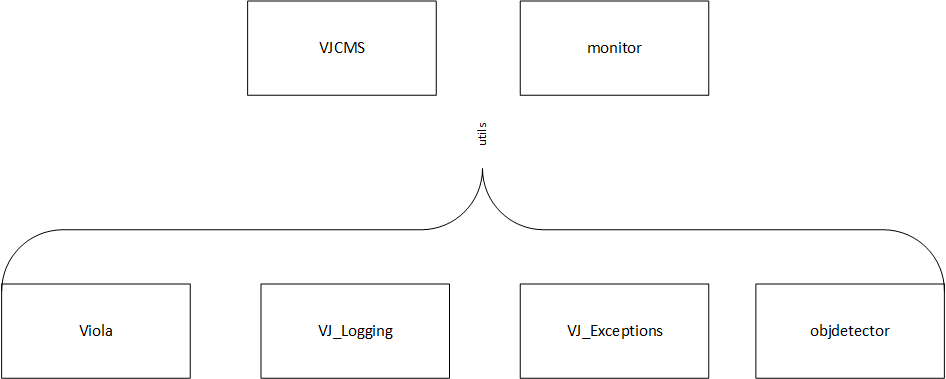
\includegraphics[width=0.7\linewidth]{img/vjcms_structure.png}
\caption{Programmaufbau}
\label{fig: structure}
\end{figure}

\subsection{VJCMS}

VJCMS bildet den Kern des Programms und übernimmt einen Großteil der Berechnungen. Neben der main-Methode befinden sich in diesem Modul Funktionen zur Ausgabe der Frames und zum Verfolgen der erkannten Objekte. Die Erkennung selbst ist wiederum in die Klasse Viola ausgelagert. 
\subsection{Viola}
\label{viola_jones}
Die Klasse Viola übernimmt die Aufbereitung der Daten des Viola-Jones Algorithmus. Der Tatsächliche Zugriff auf diese Funktionen findet in der Klasse objectdetector statt. In Viola werden die einzelnen Klassifizierer für die verschiedenen Objekte aufgerufen und die zurückgegebenen Datensätze mit den entsprechenden Labels versehen. 

\subsection{objectdetector}
Mittels dieser Klasse wird direkt auf die Funtkionalitäten von OpenCV zugregriffen und der Klassifizierer angewendet.

\subsection{VJ\_Logging}
Das Logging umfasst neben der Ausgabe auf der Konsole auch die Ausgabe in einer Datei, die im Ordner log gespeichert wird. Nachdem sowohl VJCMS als auch monitor auf diese Klasse zugreifen gibt es zwei unterschiedliche Logging-Dateien. Insgesamt gibt es 3 Arten bzw. Klassen von Meldungen, die in diesem Projekt unterschieden werden. Zum einen gibt es INFO. Hierbei handelt es sich um Meldungen die zum Beispiel angeben welche Methode gerade aufgerufen oder welcher Modus verwendet wird. Die Klasse WARNING gibt Meldungen aus, die zwar einen Fehler oder ein Problem darstellen, aber dennoch nicht zum Abbruch des Programms führen würden. Meldungen der Klasse ERROR geben Fehler oder Probleme an, die definitiv zum Abbruch oder vorzeitigen Beenden des Programmes führen. Dies muss allerdings nicht immer auf Grund einer Exception sein. In der Konsole wird kein Zeitstempel mit angegeben, sondern lediglich um welche Klasse von Meldung es sich handelt und die Meldung selbst. In dem folgenden Auszug ist eine Reihe von Logging-Ereignissen von VJCMS zu sehen. Erkannte Objekte werden ebenfalls in das Log mit eingetragen.
\begin{lstlisting}[frame=single,basicstyle=\tiny\ttfamily][H]
[Thu Feb 22 12:21:35 2018][INFO]      [main] starting program
[Thu Feb 22 12:21:35 2018][INFO]      [main] streaming to network
[Thu Feb 22 12:21:35 2018][INFO]      [main] DEBUG 1
[Thu Feb 22 12:21:35 2018][INFO]      [main] MODE 0
[Thu Feb 22 12:21:35 2018][INFO]      [main] VERBOSE 0
[Thu Feb 22 12:21:35 2018][INFO]      [detect_and_track] Begin detect_and_track
[Thu Feb 22 12:21:35 2018][INFO]      [detect_and_track] starting Thread for Viola
[Thu Feb 22 12:21:35 2018][INFO]      [detect_and_track] opening input stream
[Thu Feb 22 12:21:35 2018][OBJECT]    [Cone](351,102) (549,240)
[Thu Feb 22 12:21:35 2018][OBJECT]    [Cone](183,141) (252,180)
\end{lstlisting}

\subsection{VJ\_Exception}
Das Modul Exception enthält lediglich zwei Ausnahmeklassen. Zum einen \glqq CameraNotConnected\grqq {} und zum anderen \glqq InvalidMode\grqq .  


\subsection{monitor.py}
Monitor.py dient auschließlich der Anzeige des Streams, welcher durch VJCMS gesendet wird, falls eine Ausgabe über das Netzwerk per Parameter angegeben wurde. Dazu muss sowohl im Client als auch im Server die entsprechende IP-Adresse und Port gesetzt werden. 

\newpage
\section{Funktionalität}
\label{sec: functions}
%VJCMS besitzt im Grunde drei Modi. Zum einen $detect\_and\_track$ und zum anderen $detect$. Der erstere basiert dabei auf dem Flowchart aus Abbildung \ref{fig: vjcms_flow}. Der zweite lässt das Verfolgen der Objekte mittels Cam-Shift weg und übermittelt nur, in einem gewissen Abstand, die Koordinaten der Bounding-Boxes. Welcher Modus verwendet werden soll kann über die Option \inlinecode{python}{--mode} dem Programm mitgegeben werden. Neben diesen grundlegenen Fuktionen gibt es noch eine Reihe weitere Features, die das Skript unterstützt. Zum einen wäre da die Ausgabe eines Videostreams, mit den Bounding-Boxes. Zum einen kann dieser entweder direkt auf einen angeschlossenen Bildschirm ausgegeben werden, zum anderen besteht die Möglichkeit das Signal via TCP an einen Server zu schicken. Der Server wäre in diesem Fall das Skript monitor.py. Dies kann über die Option \inlinecode{python}{--network} angegeben werden. Die Liste aller möglichen Optionen ist in der Tabelle \ref{options}
Im Folgenden werde die einzelnen möglichen Parameter für den Funktionsaufruf aufgelistet und erklärt.
\begin{table}[H]
\begin{tabular}{|l|c|c|p{8cm}|}
\hline
Option& Wertebereich&Standard&Erklärung\\
\hline
--debug, -d & {0,1} & 1 & 0 = Als Input wird die PiCamera verwendet, 1 = Ein Video, welches im Ordner videos liegt, wird verwendet\\
\hline
--mode, -m & 0,1,2 & 0 & 0 = detect\_and\_track, 1 = detect, 2 = optimized \\
\hline 
--network, -n & 0,1,2 & 0 & 0 = Ausgabe über Monitor, 1 = Ausgabe via Stream, 2 = keine Ausgabe\\
\hline
--ip,-ip & string & local & IP-Adresse des Servers\\
\hline
--port, -port & int & 5001 & Port des Servers\\
\hline
--verbose, -v & 0,1,2 & 2 &0 = INFO, WARNING, ERROR, 1 = WARNING, ERROR, 2 = ERROR\\
\hline
--track, -t & int & 50 & Anzahl der Frames, für die ein Objekt verfolgt werden soll\\
\hline
--skip, -s & int & 5 & Anzahl der Frames, in denen der Frame ohne bearbeitung angezeigt wird\\
\hline
--object, -o & string & cone & Liste der Objekte, die erkannt werden sollen\\
\hline
--video & Boolean & False & Wenn diese Option genutzt wird, wir der aktuelle Outputstream als Video auf dem Pi gespeichert\\
\hline
\end{tabular}
\caption{Liste der Optionen für VJCMS}
\label{options}
\end{table}

VJCMS bietet eine Reihe von Funktionen, um Objekte im Videostream erkenen zu können. Es gibt insgesammt 3 Modi, die in verschiedenen Kombinationen mit anderen Paramtern genutzt werden können. Neben diesen Kernfunktionen bietet dieses Skript noch eine Reihe weitere hilfreiche Features, die vor allem für Debug-Zwecke sinnvoll sein können.
\subsection{detect\_and\_track}
In dem Modus detect\_and\_track wird alle n Frames untersucht, ob sich eines der gesuchten Objekte darin befindet. Im Anschluss werden alle in dem Frame erkannten Objekte für die Dauer von m Frames durch den Camshift Algorithmus verfolgt. Jedes Mal, wenn ein Objekt erkannt wurde, werden die Koordinaten der Bounding-Box ausgegeben.

\begin{lstlisting}[caption={Aufbau des Ergebnis-Array}]
....
{x1, y1, x2, y2, label},
{x1, y1, x2, y2, label}
....

\end{lstlisting}

Die ersten beiden Koordinaten beschreiben dabei die linke obere Ecke der Bounding-Box und das zweite Koordinaten-Paar die rechte untere Ecke. Das Label gibt an um welches Objekt es sich handelt.


\subsection{detect}
Im Gegensatz zu dem gerade eben erklärten Modus detect\_and\_track, werden hier Objekte lediglich erkannt und deren Position in dem bekannten Format ausgegeben. Es wird sonst keine weitere Bearbeitung des Frames vorgenommen. Es wird hierbei jeder einzelne Frame untersucht.

\subsection{optimized}
In diesem Modus implementieren wir einige Optimierungen, die dazu dienen sollen, die Performance des Algorithmus auf dem Pi zu verbessern.
\\
Wir nehmen an, dass in einem normalen Verkehrszenario alle für uns relevanten Schilder entweder links oder rechts von unserem Auto am Straßenrand stehen. Dies hätte zur Folge, dass sich in der Mitte unseres Bildes keine relevanten Informationen befinden. Selbst wenn ein Schild aufgrund der Distanz zu unserem Auto, theoretisch dadurch in der Mitte unseres Bilder erscheinen würde, wäre das Schild zu weit weg, als das es zur Erkennung relevant wäre.
Demzufolge könnte das mittlere Drittel des Bilder vernachlässigt werden.
In diesem Modus wird lediglich das linke und rechte Drittel eines jeden Frames untersucht, wodurch ein Teil der Berechnungen eingespart wird.

\subsection{Weitere Features}

\subsubsection{Videostream}
Wie eingangs erwähnt besteht die Möglichkeit, einen Videostream zu erzeugen, der die Bounding-Boxes anzeigt. Dazu gibt es verschiedene Ausgabemöglichkeiten. Zum einen direkt auf einem über den HDMI Port angeschlossenen Bildschirm. Zum anderen kann dieses Signal aber auch über TCP an einen entsprechenden Server geschickt werden. Dies ist mit monitor.py möglich.
Der Parameter, der dies steuert ist \inlinecode{python}{--network}.
\subsubsection{Video}
Neben der Ausgabe des Videostreames gibt es auch die Möglichkeit diesen gleich auf dem Pi als Videodatei (.avi) zu speichern. Über die Option \inlinecode{python}{--video} kann dieses Feature aktiviert werden.

\subsubsection{Debug}
Eien weitere sehr hilfreiche Option, besonders während der Entwicklung, ist der Debug Modus. In diesem Modus wird keine Kamera als Videoquelle verwendet, sondern ein Testvideo, dass sich in dem Ordner videos befindet. Dieses kann natürlich nach belieben ausgetauscht werden. Das Feature ermöglicht es einem Nutzer an verschiedenen Rechnern und Geräten zu arbeiten, ohnen einen Pi zum testen parat haben zu müssen.


%%%%%%%%%%%%%%%%
% Auswertung   %
%%%%%%%%%%%%%%%%

\chapter{Auswertung}
\chaptermark{Auswertung}
\label{chap:Asuwertung}
In einem Kurztest haben wir untersucht, wie gut die Performance des Pi's mit unserem Programm ist. Dazu haben wir eine Teststrecke aufgebaut und sind diese sowohl mit dem Pi als auch mit einem Laptopt mit angeschlossener Webcam abgefahren. 
Zum Vergleich die Spezifikationen der beiden Geräte:
\\
\\
\begin{minipage}{\linewidth}

\centering

\begin{tabular}{|c|c|}
\hline
Lenovo Yoga 13 & Raspberry Pi 3 Model b\\
\hline
\hline
Intel i5 2 x 1,8 GHz & Broadcom BCM2837 4 x 1,2 GHz\\
\hline
8 GB RAM & 1 GB RAM\\
\hline
\end{tabular}
\end{minipage}
\\
\\
In dem Test wurde der Modus 1 verwendet. D.h. es wird jedes Frame nach Objekten untersucht. Ebenfalls wurde in dem Test nach allen Objekten (Cones, Vorfahrt, Stopp Schild, Vorfahrt gewähren) gesucht. In diesem Test konnte der Pi maximal 6 FPS und der Laptop 30 FPS erzielen. 
Das gleiche Ergebnis konnte unter Verwendung des Modus 2 ereicht werden. 
Der Grund für die relativ schlechte Performance auf dem Pi liegt vermutlich am mangelnden Arbeitsspeicher. Ein weiterer Aspekt ist, dass Python-Skripte aufgrund ihres Parsings nicht performant operieren.



%%%%%%%%%%%%%%%%
%    Fazit     %
%%%%%%%%%%%%%%%%

\chapter{Fazit}
\chaptermark{Fazit}
\label{chap:Fazit}
Nach lang anhaltenden Schwierigkeiten mit dem Traingsprozess, der auf lückenhafte Dokumentation sowie nicht vorhandene Erläuterungen zur Benutzung der durch OpenCV bereitgestellten Tools zurückzuführen ist, gelang es uns für die Verkehrsschilder solide Klassifizierer zu erstellen. Die Dauer des Trainingsprozesses nahm von Objekt zu Objekt stark ab. Dauerte es noch mehrere Monate den ersten funktionierenden Klassifizierer für Pylonen zu erstellen, gelang es uns den Klassifizierer für das Vorfahrt gewähren Schild binnen weniger Stunden, inklusive der Trainingszeit für den Algorithmus, zu erstellen.\\ 
Die trainierten Klassifizierer erkennen die Verkehrsschilder mit einer sehr hohen Trefferrate aus verschiedenen Sichtwinkeln. Einziger Negativpunkt hierbei ist die auf die Kamera einfallende Lichtintensität. Ist diese zu hoch, stößt der Klassifizierer schnell an seine Grenzen. Dunkel belichteter Videoinput scheint für unsere Klassifizierer kein Problem darzustellen. Ein Grund weshalb die Verkehrsschilder gut erkannt werden können ist ihre Form. Die genutzten Weak Classifier passen gut auf die Kanten, welche bei allen drei von uns angelernten Verkehrsschildern vorkommen. Die 45\textdegree {} Kanten werden durch die Erweiterung des Modus beim Trainingsprozess als weiteres Indiz zum Erkennen genutzt, weshalb eine sehr hohe Trefferrate mit wenigen Falsepositives erreicht werden konnte.\\
Einzig die Pylonen stellen eine Besonderheit dar. Aufgrund ihrer ungewöhnlichen Form, die durch die Kanten im 70\textdegree {} Winkel zustande kommt, sowie ihrer Art der Verzerrung sollten sie von der Seite betrachtet werden, konnte kein Klassifizierer von uns erstellt werden, der Objekte eindeutig identifizieren konnte. Das Das Muster, welches vorwiegend durch den Viola-Jones Algorithmus erkannt wird, ist hierbei durch die Farbwechsel von rot zu weiß und andersherum, beziehungsweise in Graustufen auf Ebene des Algorithmus geprägt. Diese Art Muster kann je nach Belichtungsverhältnis häufig und leicht in anderen Oberflächen gefunden werden, weshalb eine sichere Nichterkennung von Falsepositives nicht gewährleistet kann. Ein weiterer Grund für potenzielle Falsepositives ist, dass die Weak Classifier nicht in ihrer vollen Funktion zum tragen kommen. Wie bereits oben erwähnt besitzen Pylonen eine steile Kante von circa 70\textdegree . Schwache Klassifizierer sind jedoch für 0\textdegree, 45\textdegree {} und 90\textdegree {} angepasst, weshalb diese im Lernprozess kaum zum Tragen kommen. Die Erkennung von Pylonen beruht somit alleinig auf dem rot-weiß Muster, welches das Charakteristikum der Eindeutigkeit gegenüber anderen Objekten, die im Alltag vorkommen, leider nicht vorweist.\\
Zusammenfassend kann gesagt werden, dass der Algorithmus nach einiger Einarbeitungszeit eine solide Basis zur Verkehrsschildererkennung darstellt und für Pylonen nur bedingt geeignet ist. Um die Erkennung von Pylonen sinnvoll zu nutzen wird vorgeschlagen weitere logische Bedingungen einzufügen, sodass ein sinnvolles Geleit durch die Pylonenpaare gewährleistet werden kann. Die Umsetzung auf dem Pi ist als erster Versuch und somit Übergangslösung anzusehen, da die gemessene Performance auf diesem Gerät nicht überzeugt.
Um diese verbessern zu können gibt es zweierlei Ansätze. Zum einen besteht die Möglichkeit eine Hochsprache für die Implementierung zu verwenden, die ein besseres Resourcenmanagement erlaubt und insgesamt performanter ausgeführt wird. Zum anderen ist eine leistungsfähigere Hardware einzusetzen. Empfehlenswert wäre an dieser Stelle die Implemenierung einzelner Schritte bzw. Berechnungen auf dem Z-Board, um besonders die rechenintensive Erkennung von Objekten zu beschleunigen. Damit sollte dann eine deutlich bessere Performance und somit ein höhere FPS Rate zu erreichen sein.


\thispagestyle{empty}
\section*{}

\newpage

%%%%%%%%%%%%
%  Anhang  %
%%%%%%%%%%%%

\begin{appendix}
\renewcommand{\chaptermark}[1]{\markboth{\uppercase{Anhang \ \thechapter.\ #1}}{}} 




\renewcommand{\chaptermark}[1]{\markboth{\uppercase{\chaptername \ \thechapter.\ #1}}{}} 

\end{appendix}








%%%%%%%%%%%%%%%%%%%%%%%%%%
%  Literaturverzeichnis  %
%%%%%%%%%%%%%%%%%%%%%%%%%%

%nicht referenzierte Literaturstellen
%\nocite{}

% Literaturverzeichnis einbinden, alpha, plain, unsrt, abbrv
\newpage
%Eintrag im Inhaltsverzeichnis
\addtocounter{page}{1}
\addcontentsline{toc}{chapter}{Literaturverzeichnis}
\addtocounter{page}{-1}

\bibliographystyle{alphadin}
\bibliography{literatur}






\end{document}
